\documentclass[tikz,border=2pt]{standalone}
\usepackage{amsmath,amssymb}
\usepackage{tikz}
\usetikzlibrary{arrows.meta}

\begin{document}
% d_2 <= d_1 <= sqrt(2) d_2 on R^2, so a taxicab ball of radius r is sandwiched between the
% Euclidean balls of radius r/sqrt(2) and r: strongly equivalent metrics.
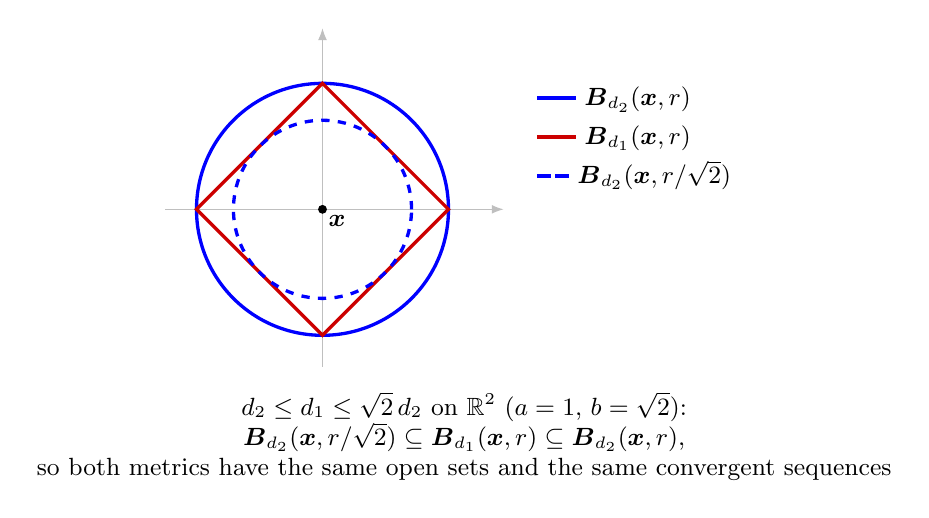
\begin{tikzpicture}[every node/.style={font=\small}]
	\draw[gray!50, -{Latex[length=1.5mm]}] (-2,0) -- (2.3,0);
	\draw[gray!50, -{Latex[length=1.5mm]}] (0,-2) -- (0,2.3);
	\draw[blue, very thick] (0,0) circle (1.6);
	\draw[red!80!black, very thick] (1.6,0) -- (0,1.6) -- (-1.6,0) -- (0,-1.6) -- cycle;
	\draw[blue, very thick, dashed] (0,0) circle (1.131);
	\fill (0,0) circle (1.6pt) node[below right, inner sep=2pt] {$\boldsymbol{x}$};
	\node[anchor=west, align=left] at (2.6,0.9) {\textcolor{blue}{\rule[2pt]{14pt}{1.5pt}}\ $\boldsymbol{B}_{d_2}(\boldsymbol{x},r)$\\[3pt] \textcolor{red!80!black}{\rule[2pt]{14pt}{1.5pt}}\ $\boldsymbol{B}_{d_1}(\boldsymbol{x},r)$\\[3pt] \textcolor{blue}{\rule[2pt]{5pt}{1.5pt}\,\rule[2pt]{5pt}{1.5pt}}\ $\boldsymbol{B}_{d_2}(\boldsymbol{x},r/\sqrt2)$};
	\node[anchor=north, align=center] at (1.8,-2.2) {$d_2\le d_1\le\sqrt2\,d_2$ on $\mathbb{R}^2$ ($a=1$, $b=\sqrt2$):\\ $\boldsymbol{B}_{d_2}(\boldsymbol{x},r/\sqrt2)\subseteq\boldsymbol{B}_{d_1}(\boldsymbol{x},r)\subseteq\boldsymbol{B}_{d_2}(\boldsymbol{x},r)$,\\ so both metrics have the same open sets and the same convergent sequences};
\end{tikzpicture}
\end{document}
